\documentclass{article}

\usepackage[english]{babel}
\usepackage[utf8]{inputenc}
\usepackage{kpfonts}
\usepackage[left=2.8cm, right=2.8cm, top=2.8cm, bottom=3cm]{geometry}
\usepackage{titling}
\usepackage{graphicx}
\usepackage{hyperref}

\graphicspath{{ims/}}

%%%%%%%%%%%% Title Part %%%%%%%%%%%%
\pretitle{
	\begin{center}
	\includegraphics[width=4cm]{logo_ens_lyon.pdf}
	\hspace{5cm}
	
\includegraphics[width=5.5cm]{logo_tu_delft.png}
	\LARGE
}
\title{
	\rule{\linewidth}{0.4mm}
	\textbf{Perspective Check in Paintings} \\
	\textit{M1 Internship}
	\rule{\linewidth}{0.6mm}
}
\author{
	Yoann Coudert--Osmont \\[3mm]
	\textit{Supervised by} \\
	Elmar Eisemann \qquad Ricardo Marroqium \\[2mm]
}
\date{May - July 2019}
%%%%%%%%%%%%%%%%%%%%%%%%%%%%%%%%%%%%

\begin{document}
	\maketitle
	
	\section*{Introduction}
	
	\begin{figure}
		\centering
		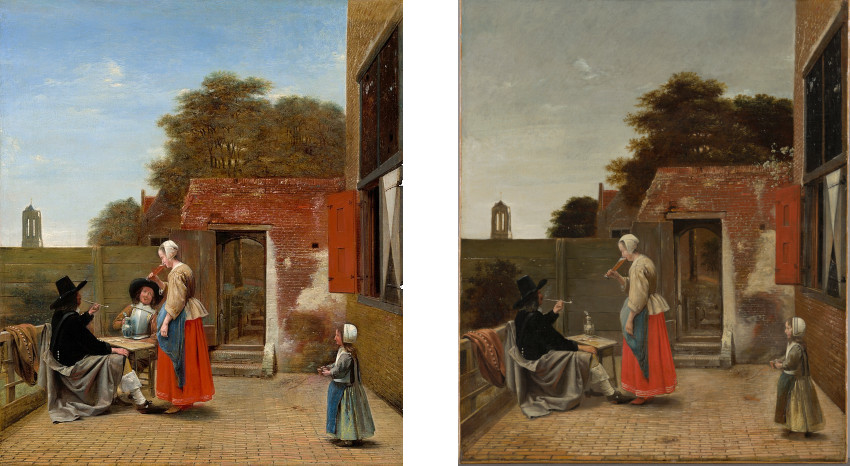
\includegraphics[scale=1.25]{paintings_pair.jpg}
		\caption{A pair of similar paintings}
		\label{im:pair}
	\end{figure}

	In a Delft museum, paintings by Pieter de Hooch are on display. It is quite easy to notice that some pairs of paintings are very similar (e.g. \figurename \ref{im:pair}). One hypothesis that would explain this strangeness is the possibility that another painter copied Pieter de Hooch's paintings. Looking at the pairs in more detail, we can notice that quite often one painting respects the rules of perspective well and the other does not respect them. This gives credibility to the hypothesis of the existence of another painter. But the human tends to be biased to check that in each pair one painting respects the rules of perspective and the other does not. Then comes the need to create a tool to check whether the perspective is respected in a painting with as little human intervention as possible. The goal of this internship was therefore to create a graphical interface to verify the perspective in a painting with as much automation as possible. \\
	Tools already exist to find lines in an image. The most common and the one I used is the Hough transform \cite{hough}. I will describe the algorithms used to create my interface in this report. The development of a graphical user interface with minimal user control was necessary because there is no guarantee that a fully automated program will do exactly what you want. Much of the internship was used to learn how to make a graphical interface with Qt and to design an interface that is easily usable. But I'm not going to describe how this interface works, I'll just give some implemented features at the end of the report.

	\begin{center}
		\tableofcontents
	\end{center}
	
	\newpage
	
	\section{Reminders on the rules of perspective}
	
	The main rule of perspective is that when you make a drawing, the parallel lines must all cross at the same point. We call this point a vanishing point. In addition, all vanishing points must be on the same line. This line is the vanishing line and corresponds to the horizon.
	
	\section{Description of the algorithm}
	
	% Need to talk about what I tried before hough transform (PCA on connex components)

	\subsection{General description}
	
	\subsection{Smoothing}
	
	\subsection{Gradient}
	
	\subsection{Hough Transform}
	
	\begin{figure}[h]
		\centering
		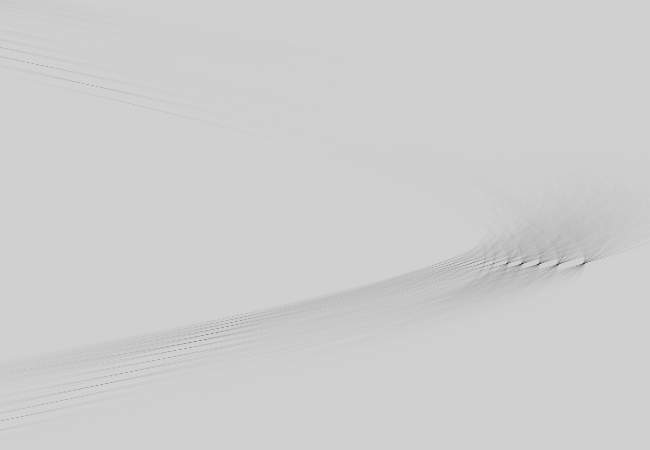
\includegraphics[scale=1.2]{hough_painting.png}
		\caption{Hough Transform}
	\end{figure}

	\section{Attempt to redraw the paintings with a perfect perspective}

	\section{Conclusion}
	
	As a conclusion I did nothing during this internship !
	
	\appendix
	
	\section{Source Code}
	
	Here is my git repository: \url{https://github.com/Nanored4498/Painting-Analysis}.

	\bibliographystyle{alpha}
	\bibliography{bib.bib}
	
\end{document}